\documentclass[tikz]{standalone}
\begin{document}
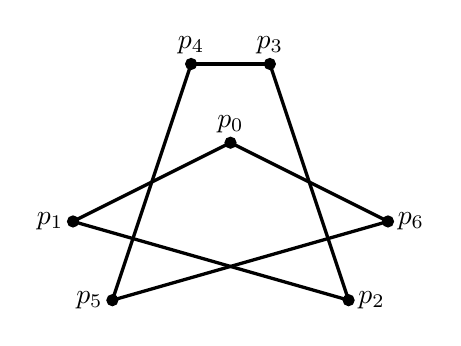
\begin{tikzpicture}


    \filldraw[black] (0, 0) coordinate(p0) circle (2pt) node[above] {$p_0$};
    \filldraw[black] (-2,-1) coordinate(p1) circle (2pt)  node[left] {$p_1$};
    \filldraw[black] (1.5,-2) coordinate(p2) circle (2pt)  node[right] {$p_2$};
    \filldraw[black] (0.5,1) coordinate(p3) circle (2pt)  node[above] {$p_3$};
    \filldraw[black] (-0.5,1) coordinate(p4) circle (2pt)  node[above] {$p_4$};
    \filldraw[black] (-1.5,-2) coordinate(p5) circle (2pt)  node[left] {$p_5$};
    \filldraw[black] (2,-1) coordinate(p6) circle (2pt)  node[right] {$p_6$};
    
    
    \draw[very thick] (p0) -- (p1);
    \draw[very thick] (p1) -- (p2);
    \draw[very thick] (p2) -- (p3);
    \draw[very thick] (p3) -- (p4);
    \draw[very thick] (p4) -- (p5);
    \draw[very thick] (p5) -- (p6);
    \draw[very thick] (p6) -- (p0);

\end{tikzpicture}
\end{document}